	
\subsection{Information Theory and Spatial Structure}
	Two of the most fundamental objects of information theory are the entropy of a single random and the mutual information of two. Let $X$ be a spatial variable, such as a set of coordinates in space or a neighborhood name. Let $Y$ be a compositional variable that we aim to study, defined on an alphabet $\mathcal{Y}$. In the simple case in which $\mathcal{Y}  = \{\text{Black, White}\}$, Figure \ref{fig:toy} illustrates a range of possible joint distributions $p(X,Y)$. Comparing the completely undiverse city (a) and the spatially uniformly diverse (b) motivates the first fundamental information measure, the entropy:
	\begin{equation}
		H(Y) \triangleq \sum_{y \in \mathcal{Y}} p(y) \log p(y)\;.
	\end{equation}
	The entropy measures how evenly the global marginal distribution $p(Y)$ is distributed over the alphabet $\mathcal{Y}$. It thereby clearly distinguishes cities (a) and (b): since (a) is completely uniform, $H_a(Y) = 0$, while $H_b(Y) \neq 0$. On the other hand, the entropy $H$ is unable to distinguish between the spatial uniformity of (b) and the spatially variability of (c). To distinguish these two cities we may use the mutual information, which is defined in terms of the Kullback-Leibler divergence $D$:
	\begin{align}
		D[p(Z)\|q(Z)] &\triangleq \sum_z p(z) \log \frac{p(z)}{q(z)} \\
		I(X,Y) &\triangleq D[p(X,Y) \| p(X)p(Y)] = \E_X[D[p(Y|X)\|p(Y)]]
	\end{align}
	The divergence $D$ is (with some caveats) a measure of distance in the space of probability distributions, and so $I(X,Y)$ may be interpreted as the distance between the true joint distribution $p(X,Y)$ and the product of marginals $p(X)p(Y)$. Since the latter expresses statistical independence between $X$ and $Y$, $I(X,Y)$ measures the extent to which $X$ and $Y$ are dependent. In city (b), $X$ and $Y$ are independent: knowing $X$ (where an individual lives) conveys no information about that $Y$ (that individual's race).  In city (c), on the other hand $X$ and $Y$ are completely dependent: if you know where someone lives, you know their race with 100\% confidence. 

	City (d) shares with city (c) the fact that residence and race are maximally dependent. However, city (d) embodies the ``checkerboard problem'': measures that use only the joint distribution $p(X,Y)$ without additionally considering the spatial information contained within $X$ will evaluate city (d) to be the same as city (c), despite their considerably different patterns of racial separation and potentially very different implications for planning and policy. A recent working paper \cite{Roberto2015} provides one highly operational approach to this problem, using road network topology and a weighting function that decays with distance to define a localized measure based on the Kullback-Leibler divergence. Here we pursue an alternative strategy, showing that a localization of the mutual information both measures spatial variation in race and corresponds to the estimation of a fundamental statistical property of the distribution $p(X,Y)$. 


	\begin{figure}
		\centering
		  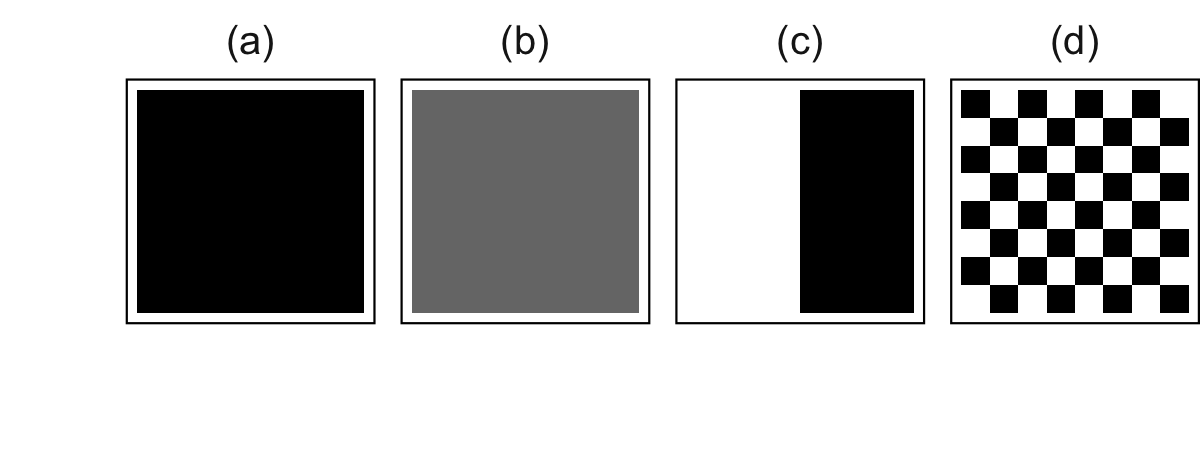
\includegraphics[width=.7\linewidth]{figs/checkerboard.png}
		  \begin{tabular}{c | c c c}
			  City & $H(Y)$ & $I(X,Y)$ & $J(X,Y)$ \\
			  \hline			
			  (a) & 0.0 & 0.0 & 0.0\\
			  (b) & 0.7 & 0.0 & 0.0\\
			  (c) & 0.7 & 0.7 & 0.6\\
			  (d) & 0.7 & 0.7 & 2.7\\
			  \hline  
			\end{tabular}
		\caption{Information theory and the checkboard problem: model cities with various kinds of spatial diversity can be distinguished through progressively more subtle spatial information measures.}
		\label{fig:toy}
		\end{figure}

\subsection{Measuring Socio-Spatial Complexity}
		To motivate our methods, we first consider an idealized scenario in which we have a differentiable field $p(y|x)$ of observed probability distributions for each $x \in M \subset \R^n$, where $M$ is interpretable the ``map'' on which we work. 

		Fix a point $x_0 \in M$ and a radius $r > 0$. Let $B_r(x_0)$ denote the ball of radius $r$ about $x_0$. Then, define the \emph{local mutual information in radius $r$} as the mutual information between $X$ and $Y$, restricted to the small ball $B_r(x_0)$ about $x_0$:
		\begin{equation}
			I_r(x_0) \triangleq \E_X[D[p(\cdot|X)\| p(\cdot|X \in B_r(x_0))]|X \in B_r(x_0)] \label{eq:local}
		\end{equation}
		Intuitively, $I_r(x_0)$ measures how much the probability field $p(y|x)$ varies with $x$ in a small neighborhood of $x_0$. It is therefore a natural measure of local complexity, aligned in approach with the global mutual information but designed to detect pattern in local variations. As expected, $I_r(x_0) = 0$ if and only if $p(y|x)$ is constant for each $y$ in the ball $B_r(x_0)$; that is, if within $B_r(x_0)$ the field $p(y|x)$ resembles toy city (b) in Figure \ref{fig:toy}. 

		\begin{figure}
			\centering
			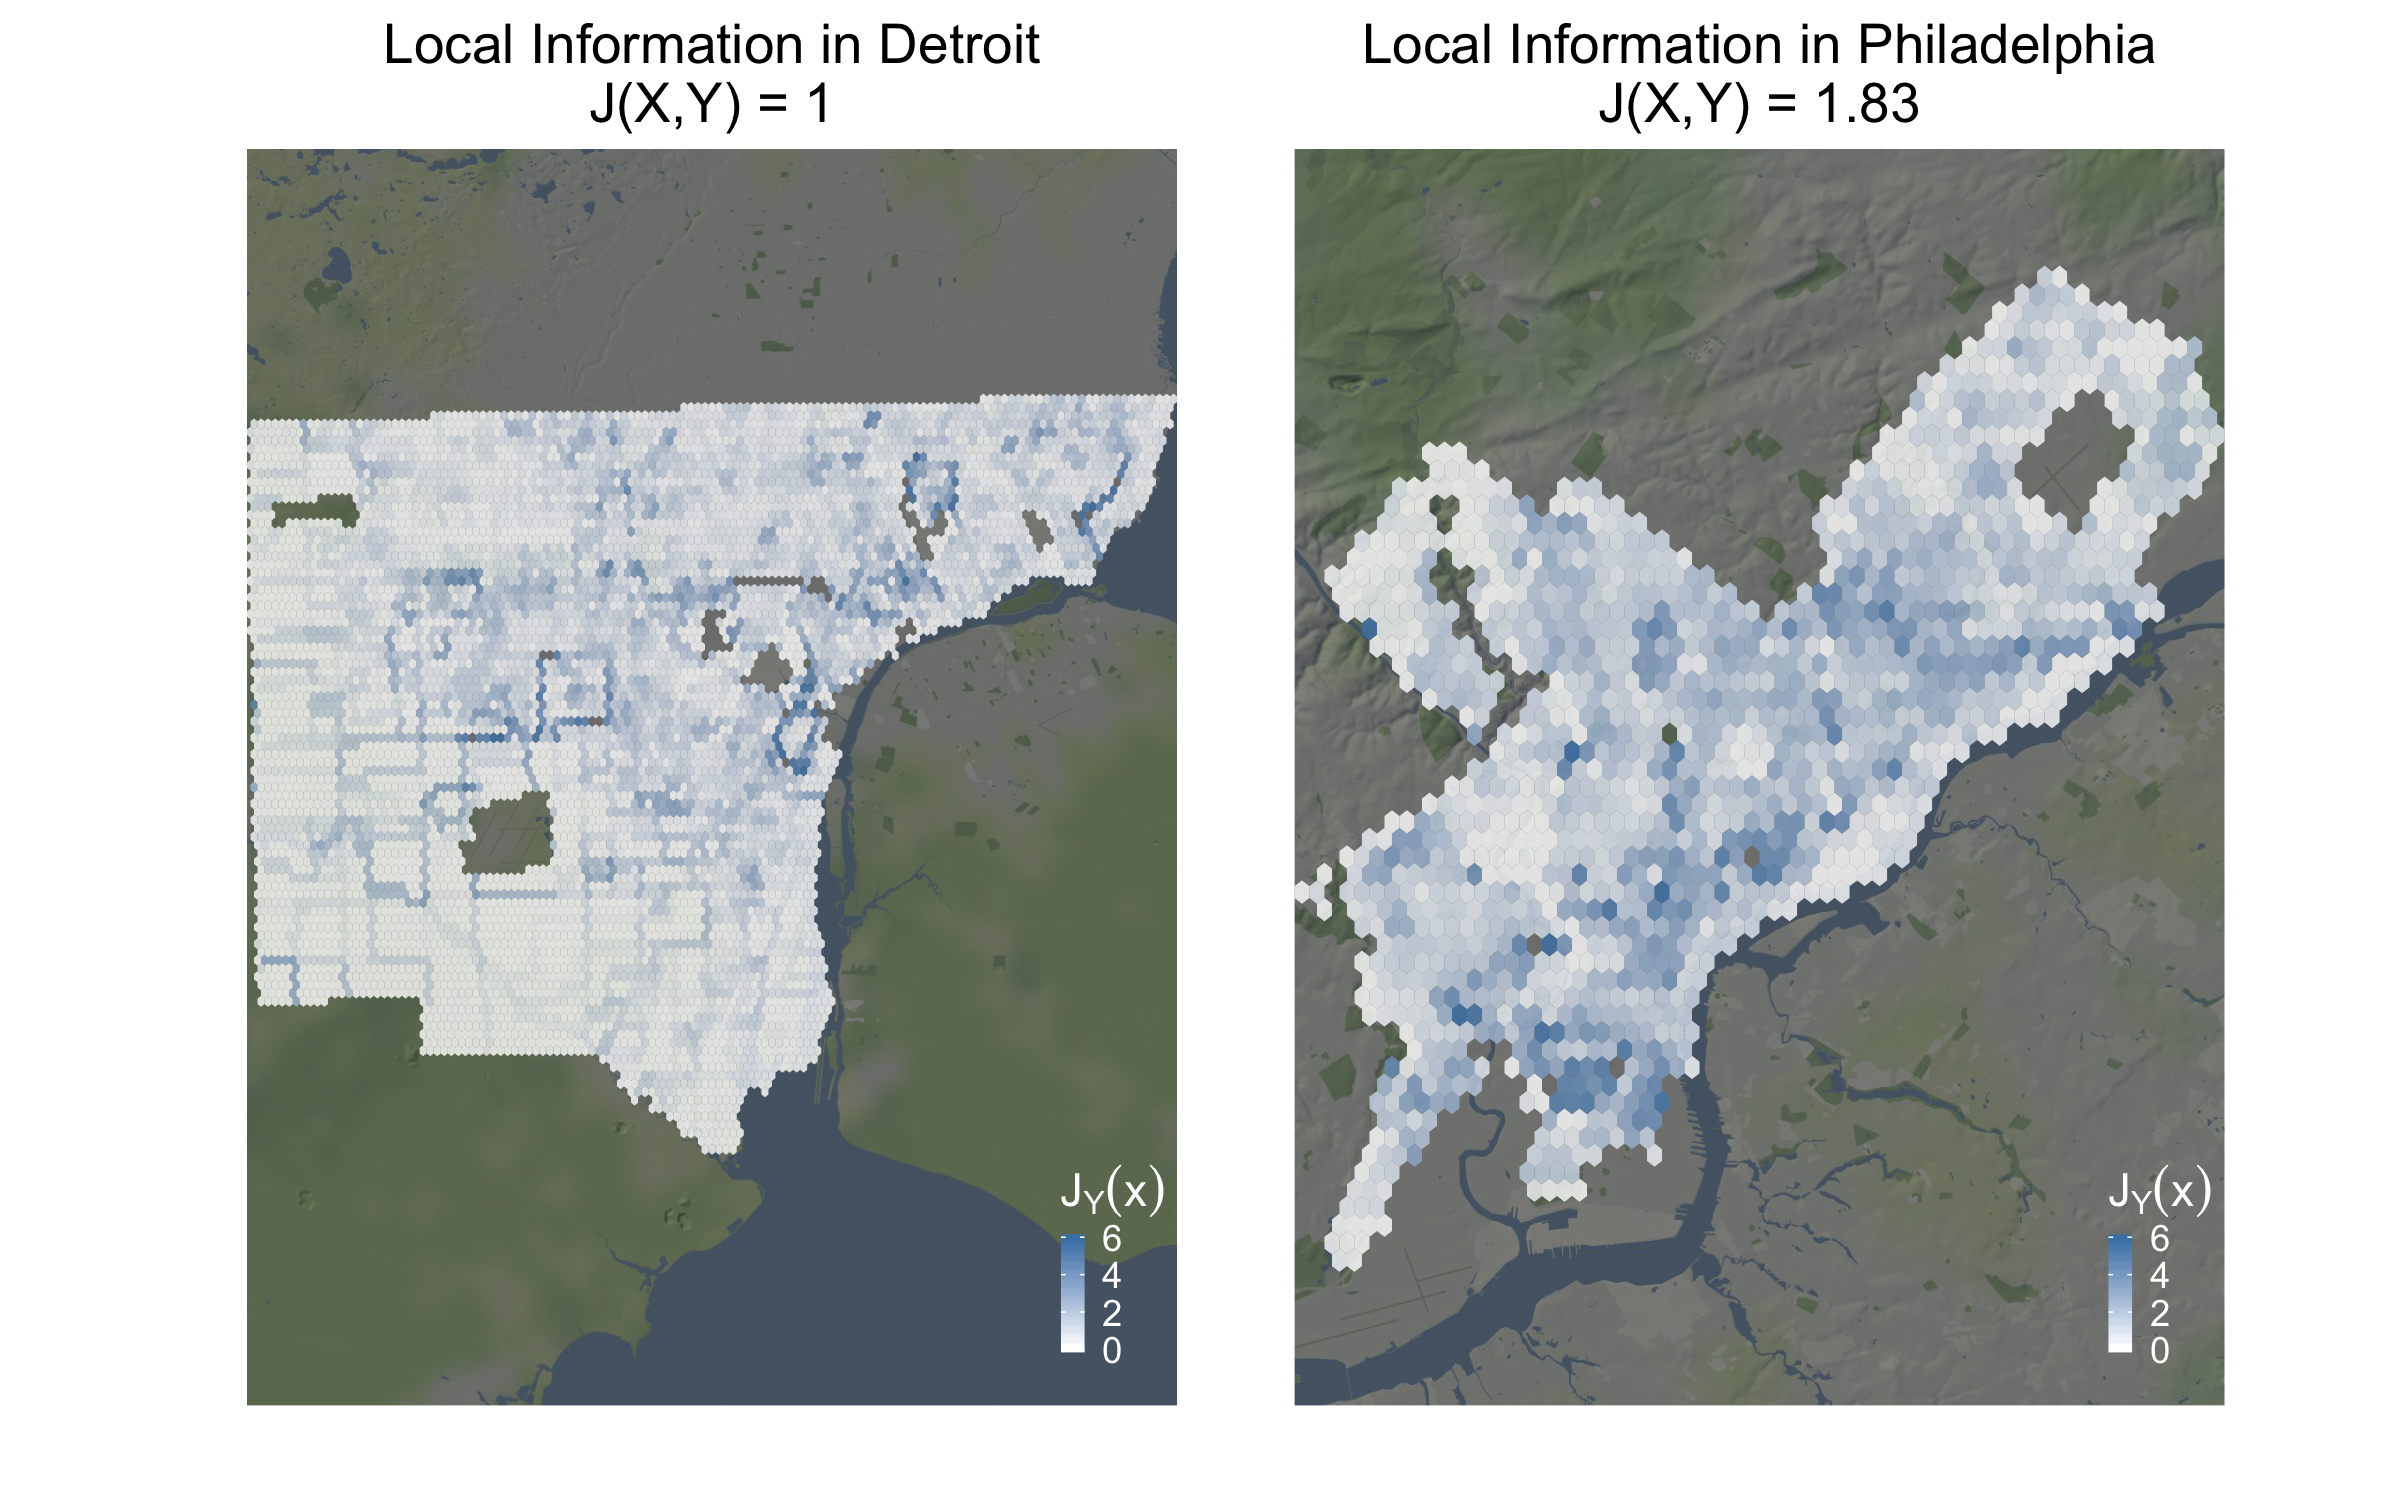
\includegraphics[width=.5\textwidth]{figs/method_illustration.png}
			\caption{Illustration of methodology for estimating local information in Suffolk County, MA (Boston). We first cover the map in a hexgrid, and compute the mutual information within each hex from the Census tracts that overlap the hex, weighted by density. }
			\label{fig:method}
		\end{figure}

		In the definition \eqref{eq:local}, $r$ may be thought of as the spatial resolution at which we conduct analysis, and $I_r(x_0)$ is highly dependent on $r$. However, it is possible to show that $I_r(x_0)$ is related to a fundamental statistical property of the probability field $p(y|x)$ that is resolution-independent. Under the stated conditions, the following approximation holds: 

		\begin{equation}
			\frac{I_r(x)}{r^2} \cong \frac{1}{4} \text{trace} (J_Y(x))\;, \label{approx}
		\end{equation}
		where $J_Y(x)$ is the Fisher information matrix in $Y$ about $x$, defined as 
		\begin{equation}
			J_Y(x) \triangleq \E_Y\left[ (\nabla_x \log p(Y|x))(\nabla_x \log p(Y|x))^T \right]\;.
		\end{equation}
		A more formal statement and proof of \eqref{approx} are provided in Appendix 2. The Fisher information $J_Y$ is a fundamental quantity in statistics and information theory. From a geometric perspective, $J_Y$ provides the natural intrinsic metric in the geometric space of probability distributions parameterized by the spatial variable $x$. Equation \eqref{approx} therefore expresses a relationship between the local mutual information $I_r(x)$ and the information geometry of the underlying probability field. Corresponding to the fact that $I_r(x_0)$ vanishes if and only if $p(y|x)$ is constant in $B_r(x_0)$, $J_Y(x_0) = 0$ if and only if $\nabla_x p(y|x_0) = 0$ for all $y$. This implies that $x_0$ is a stationary point, about which the probability field $p(y|x_0)$ exhibits only small (2nd order or smaller) changes with respect to changes in $x$. 

		Since the Fisher information is a strictly local measure of statistical variability around $x$, we can aggregate the Fisher information to derive a measure of average local variability. The \emph{mean local information} is 
		\begin{equation}
		J(X,Y) \triangleq \E_X[\text{trace }J_Y(X)]
		\end{equation} 
		We propose the aggregate quantity $J(X,Y)$ as a third  measure--alongside the entropy $H(Y)$ and mutual information $I(X,Y)$-- as a tool for the information-theoretic structure of spatial compositional complexity. 
	\subsection{Identifying Natural Neighborhoods}
		Suppose that we have a collection of tracts labeled with the random variable $X$, and suppose that each tract has an additional label $C$ denoting the \emph{cluster} in which it lies. Then, it is possible to show that 
		\begin{equation}
			I(X,Y) = I(Y,C) + I(X,Y|C) \label{eq:information_decomp}
		\end{equation}
		Equation \eqref{eq:information_decomp} has a natural interpretation: the information I have about $Y$ if I know $X$ is equal to the  information I have if I know the cluster $C$, plus the amount of information I have if I subsequently learn the exact location $X$. Usefully, equation \eqref{eq:information_decomp} decomposes the system-wide mutual information $I(X,Y)$ into a \emph{between-cluster} component $I(Y,C)$ and an \emph{within-cluster} component $I(X,Y|C)$. It is therefore comparable to various ``sum of squares'' decompositions that frequently appear in classical statistics. Indeed, it is possible to show that, when the differences between locations are small, the mutual information can be interpreted as a variance, in which case \eqref{eq:information_decomp} expresses the sum of squares composition directly. 

		Finally, equation \eqref{eq:information_decomp} motivates a natural, information-based scheme for identifying natural neighborhoods. If all I had access to were the cluster labels $C$ and not the locations $X$, then my information would be $I(Y,C)$. A ``good'' clustering therefore maximizes the between-cluster information $I(Y,C)$, which entails minimizing the within-cluster information $I(X,Y|C)$. Solving this problem exactly is a challenging discrete optimization problem, and may not be computationally tractable. We can, however, construct a greedy algorithm with good performance. Suppose that we face the problem of choosing a collection $I = \{1,2,\ldots\}$ of locations to cluster together. The reduction in information associated with aggregating the locations $I$ into a single cluster is 
		\begin{align}
			d(I) \triangleq  \sum_{i \in I} p(X = i)D[p(Y|X = i)\| p(Y|X \in I)] - p(X\in I)D[p(Y|X\in I) \| p(Y)] \label{eq:info_dist}
		\end{align}
		where $p(Y) = \sum_{x} p(x,Y)$ is the global marginal distribution. If we choose $I = \{i,j\}$, then equation \eqref{eq:info_dist} defines a natural information distance between locations $i$ and $j$. Like the KL divergence, this distance is strictly nonnegative; unlike the KL divergence, this distance is symmetric. Importantly, we can therefore use the distance $d(i,j)$ as a dissimilarity measure for the purposes of clustering. Our greedy procedure is simple: at each stage, the algorithm aggregates together two locations $i$ and $j$ such that 
		\begin{enumerate}
			\item Locations $i$ and $j$ are adjacent in space. This requirement ensures that the results may be naturally understood as neighborhoods, rather than disparate tracts with similar demographics.  
			\item Among all adjacent pairs, $d(i,j)$ is the smallest possible. 
		\end{enumerate}
		This greedy procedure defines a form of agglomerative hierarchical clustering distinguished by two characteristics: its spatial constraints and its pursuit of minimal information loss at each step. As a greedy algorith, it possesses no guarantees for optimal solutions, but in practice its performance leads to intuitive neighborhoods. 

	
